%% Seção 7: A Linguagem como Ferramenta de Diagnóstico e Intervenção na Busca pela Autenticidade

\chapter{A Linguagem como Ferramenta de Diagnóstico e Intervenção na Busca pela Autenticidade do Ser}

\epigrafe{A alma humana é um abismo.}{Fiódor Dostoiévski, \textit{Crime e Castigo}}

\textbf{7.} A linguagem é tanto ferramenta de diagnóstico quanto de intervenção, permitindo ao paciente explorar as profundezas de sua subjetividade e buscar a autenticidade do ser.

\section{Linguagem e estado mental profundo}

\textbf{7.1} A linguagem reflete o estado mental profundo do indivíduo, revelando conflitos internos e questionamentos existenciais.

\begin{tese}
Se a linguagem expressa as camadas mais profundas da subjetividade (conforme Dostoiévski), então ela pode ser utilizada para diagnosticar conflitos internos e dilemas existenciais.
\end{tese}

\begin{hipotese}[title=Hipótese 7.1.1 (Condicional)]
Se o paciente utiliza a linguagem para expressar angústias e contradições, então esses elementos podem ser analisados para compreender seu estado mental.
\end{hipotese}

\begin{referencia}[title=Referência a Dostoiévski]
Em obras como \textit{Crime e Castigo}, Dostoiévski explora os conflitos internos de seus personagens, revelando através da linguagem seus dilemas morais e psicológicos.
\end{referencia}

\begin{aforismo}
Nas palavras que confessam, a alma revela seus abismos.
\end{aforismo}

\section{Fragmentação e ambiguidade na linguagem}

\textbf{7.2} A linguagem pode ser fragmentada e ambígua, refletindo a complexidade da mente e a luta pela autocompreensão.

\begin{tese}
Se a linguagem fragmentada reflete a fragmentação interna (conforme Kafka), então ela pode ser utilizada para diagnosticar estados de alienação e desintegração psíquica.
\end{tese}

\begin{referencia}[title=Referência a Kafka]
Em \textit{A Metamorfose} e outros contos, Kafka utiliza uma linguagem que transmite a alienação e o absurdo da existência humana.
\end{referencia}

\begin{aforismo}
No discurso que se perde em labirintos, o eu busca uma saída para si mesmo.
\end{aforismo}

\section{Desconstrução e reinterpretação da linguagem}

\textbf{7.3} A linguagem é uma construção que pode ser desconstruída e reinterpretada, permitindo a transformação do indivíduo.

\begin{tese}
Se a linguagem pode ser desconstruída para revelar novas significações (conforme Nietzsche), então ela pode ser utilizada como ferramenta de intervenção para transformar a subjetividade.
\end{tese}

\begin{referencia}[title=Referência a Nietzsche]
Em \textit{Assim Falou Zaratustra} e \textit{Além do Bem e do Mal}, Nietzsche propõe a transvaloração dos valores e a necessidade de criar novos significados, rompendo com padrões estabelecidos.
\end{referencia}

\begin{aforismo}
Ao romper as correntes das palavras antigas, o espírito se liberta para criar seu próprio caminho.
\end{aforismo}

\section{Exploração da interioridade através da linguagem}

\textbf{7.4} A linguagem é veículo para a exploração da interioridade e das emoções mais profundas.

\begin{tese}
Se a linguagem permite a exploração das emoções e da interioridade (conforme Clarice Lispector), então ela é essencial no processo terapêutico de autodescoberta.
\end{tese}

\begin{referencia}[title=Referência a Clarice Lispector]
Em obras como \textit{A Paixão Segundo G.H.} e \textit{A Hora da Estrela}, Lispector explora a interioridade de suas personagens, utilizando uma linguagem intimista e introspectiva.
\end{referencia}

\begin{aforismo}
Nas palavras que sussurram o indizível, encontra-se a essência do ser.
\end{aforismo}

\section{Confronto com conflitos internos e transcendência}

\textbf{7.5} A linguagem é o meio pelo qual o paciente pode confrontar e transcender seus conflitos internos, alcançando a autenticidade.

\begin{tese}
Se a linguagem permite ao indivíduo confrontar seus conflitos e contradições (conforme Dostoiévski e Kafka), então ela é essencial para a intervenção terapêutica que busca a autenticidade do ser.
\end{tese}

\begin{aforismo}
Ao dar voz aos silêncios da alma, o ser encontra seu verdadeiro tom.
\end{aforismo}

%% DIAGRAMA DA SEÇÃO 7
\section*{Diagrama Representativo: Linguagem como Diagnóstico e Intervenção}

\begin{center}
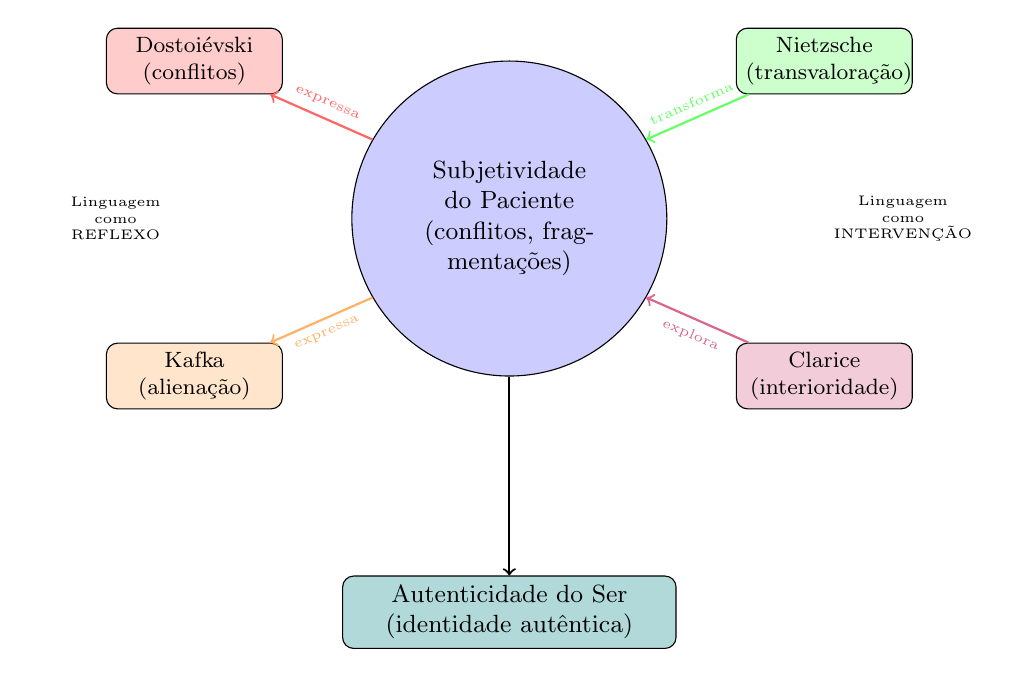
\begin{tikzpicture}[scale=1, every node/.style={font=\small}]
    % Círculo central - Subjetividade
    \node[draw, circle, fill=blue!20, minimum size=4cm, text width=3cm, align=center] (subj) at (0,0) {Subjetividade\\do Paciente\\(conflitos, fragmentações)};

    % Autores ao redor
    \node[draw, rounded corners, fill=red!20, text width=2cm, align=center, font=\footnotesize] (dost) at (-4,2) {Dostoiévski\\(conflitos)};
    \node[draw, rounded corners, fill=orange!20, text width=2cm, align=center, font=\footnotesize] (kafka) at (-4,-2) {Kafka\\(alienação)};
    \node[draw, rounded corners, fill=green!20, text width=2cm, align=center, font=\footnotesize] (nietz) at (4,2) {Nietzsche\\(transvaloração)};
    \node[draw, rounded corners, fill=purple!20, text width=2cm, align=center, font=\footnotesize] (clarice) at (4,-2) {Clarice\\(interioridade)};

    % Setas de reflexão (linguagem como reflexo)
    \draw[thick, ->, red!60] (subj.150) -- node[above, sloped, font=\tiny] {expressa} (dost);
    \draw[thick, ->, orange!60] (subj.210) -- node[below, sloped, font=\tiny] {expressa} (kafka);

    % Setas de intervenção (linguagem como ferramenta)
    \draw[thick, ->, green!60] (nietz) -- node[above, sloped, font=\tiny] {transforma} (subj.30);
    \draw[thick, ->, purple!60] (clarice) -- node[below, sloped, font=\tiny] {explora} (subj.330);

    % Resultado
    \node[draw, rounded corners, fill=teal!30, text width=4cm, align=center] (auth) at (0,-5) {Autenticidade do Ser\\(identidade autêntica)};

    \draw[thick, ->] (subj) -- (auth);

    % Labels
    \node[font=\tiny, text width=2cm, align=center] at (-5,0) {Linguagem\\como\\REFLEXO};
    \node[font=\tiny, text width=2cm, align=center] at (5,0) {Linguagem\\como\\INTERVENÇÃO};
\end{tikzpicture}
\end{center}

\begin{sintese}[title=Síntese Final da Seção 7]
A linguagem é tanto ferramenta de diagnóstico quanto de intervenção, permitindo ao paciente explorar as profundezas de sua subjetividade e buscar a autenticidade do ser. Conforme Nietzsche, a desconstrução e ressignificação da linguagem possibilitam a transformação pessoal. Kafka e Dostoiévski mostram que a linguagem pode refletir a fragmentação interna e os conflitos existenciais, servindo como meio para confrontá-los e superá-los. Clarice Lispector evidencia como a linguagem pode ser veículo para a exploração da interioridade e das emoções mais profundas.

O terapeuta, ao compreender e interpretar a linguagem do paciente, pode diagnosticar estados internos e guiar a intervenção terapêutica. Ao incentivar o paciente a expressar seus conflitos e a reestruturar suas narrativas, promove-se a integração cognitiva e emocional, levando à construção de uma identidade autêntica.
\end{sintese}

\nextpage
